%% img/ExpvsExppvsPSpace.tex
%% Copyright 2019 Andrea Berlingieri
%
% This work may be distributed and/or modified under the
% conditions of the LaTeX Project Public License, either version 1.3
% of this license or (at your option) any later version.
% The latest version of this license is in
%   http://www.latex-project.org/lppl.txt
% and version 1.3 or later is part of all distributions of LaTeX
% version 2005/12/01 or later.
%
% This work has the LPPL maintenance status `maintained'.
%
% The Current Maintainer of this work is Andrea Berlingieri.
%
% This work consists of all files listed in manifest.txt
\documentclass{standalone}

\usepackage{../TikzStyle}
\usepackage{../mystyle}
\usetikzlibrary{automata}

\newcommand{\gpoint}[2]{%
\filldraw [gray] (#1,#2) circle [radius=2pt]
}

\begin{document}
    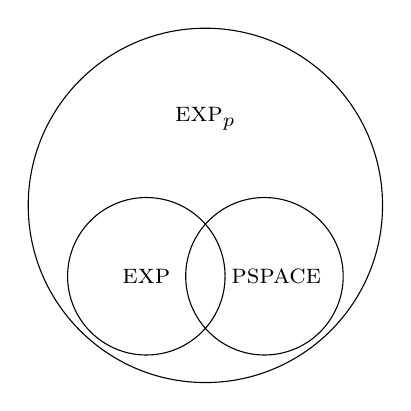
\begin{tikzpicture}
        %\node[draw,circle,inner sep=0.5cm] () at (0,0) {$\PClass$};
        \draw (-0.75,0) circle [radius=1cm];
        \draw (0.75,0) circle [radius=1cm];
        \draw (0,0.9) circle [radius=2.25cm];
        \node () at (-0.75,0) {$\textsc{exp}$};
        \node () at (0.9,0) {$\textsc{pspace}$};
        \node () at (0,2) {$\textsc{exp}_{p}$};
    \end{tikzpicture}
\end{document}
